\title{Computer Vision}
\author{
        Assignment 2 - Canny Edge Detection\\
Spring 2023
}
\date{}
\documentclass[12pt]{article}
\usepackage[margin=0.7in]{geometry}
\usepackage{graphicx}
\usepackage{float}
\usepackage{amsmath}


\begin{document}
\maketitle


\section*{Introduction}
In this assignment you will demonstrate your ability to implement the individual components of a Canny Edge Detector\\

\noindent
In this assignment, as with all of our assignments, you shouldn't be using built-in functions that violate the ``spirit'' of the assignment.  For instance, in part 2, you can't use a function like \emph{conv2} or \emph{imgaussfilt} nor an \emph{edge} function anywhere.  Use your intuition, and when in doubt ask the instructor or TA.\\

\noindent
In this assignment you will demonstrate your ability to:
\begin{itemize}
\item Create and apply smoothing and gradient kernels.
\item Find edge candidates by thresholding based on gradient strength.
\item Apply non-maximum suppression.
\item Apply hysteresis.

\end{itemize}

\section*{Grading}
\begin{table}[h]
\begin{centering}
\begin{tabular}{|l|l|}
\hline
Theory Questions & 20pts \\
Gaussian Smoothing & 20pts\\
Computing Gradients & 20pts\\
Non-maximum supression & 10pts\\
Hysterisis & 20pts\\
Apply pipeline to addition image & 10pts\\
\hline
\textbf{TOTAL} & 100pts\\
\hline
\end{tabular}
\caption{Grading Rubric}
\end{centering}
\end{table}

\newpage
\section*{Dataset}
For this assignment we are going to implement the various stages of a Canny Edge Detector and apply them to a few images, observing the results along the way.\\

\noindent
I have provided a single sample image, \emph{circles1.gif}, for us to observe the effect of stages of the edge detector.   In addition, use an image of your choosing to apply the Canny Edge Detector pipeline to as well to verify its robustness.

\newpage
\section{(26pts) Theory Questions}
\begin{enumerate}
\item (5pts) Apply a $3\times3$ mean filter to the following 2D matrix.  You may assume that the filter is only applied to areas of the data that have a full 9 samples to process.  Feel free to use Matlab to help you compute this, however, realize that you may be asked to do this without a calculator on an exam.  \textbf{Leave your answers as floating point values, with a single digit after the decimal point}.
$$ I=\begin{bmatrix}	7&     7&     6&     3&     3&     4&     2&     2\\
							3&     7&     2&     6&     4&     4&     5&     7\\
							5&     4&     7&     5&     1&     1&     2&     2\\
							2&     1&     3&     4&     1&     3&     5&     6\\
							6&     2&     2&     7&     4&     2&     5&     4\\
							2&     2&     2&     3&     6&     6&     6&     7\\
							4&     6&     5&     6&     7&     3&     4&     1\\
							5&     2&     4&     6&     1&     4&     1&     4\\
\end{bmatrix}$$\\
Ans: To apply a 3 × 3 mean filter to the given 2D matrix, we need to convolve the matrix with a 3 × 3 kernel that has all elements equal to 1/9. The convolution operation involves sliding the kernel over the matrix and computing the average of the products of corresponding elements of the kernel and matrix at each position.\\

To apply this filter to matrix I using conv2 we can use the following code in MATLAB:\\

meanfilter = ones(3)/(3\^{}2);\\
J = conv2(I, meanfilter,'valid');\\
J = round(J,1);\\

Here, ones(3)/(3\^{}2) creates a kernel with all elements equal to 1/9. The 'valid' option in conv2 returns only those parts of the convolution that are computed without zero-padded edges. Finally, round(J,1) rounds the resulting matrix to one decimal place.\\

$$ J=\begin{bmatrix}	5.3&     5.2&     4.1&     3.4&     2.9&    3.2&\\
						3.8&     4.3&     3.7&     3.2&     2.9&    3.9&\\
					    3.6&     3.9&     3.8&     3.1&     2.7&    3.3&\\
						2.4&     2.9&     3.6&     4&       4.2&    4.9&\\
						3.4&     3.9&     4.7&     4.9&     4.8&    4.2&\\
						3.6&     4&       4.4&     4.7&     4.2&    4&\\
\end{bmatrix}$$\\

\item (5pts) What is the kernel function for a $5\times5$ Gaussian function with $\sigma=2$?   Normalize the kernel so that its elements sum to one. \\
Ans: the kernel function for a 5 × 5 Gaussian function with $\sigma = 2$:\\

W (i,j) $\propto e{-\frac{(i-(k+1))^2 + (j-(k+1))^2}{2\sigma^2}}$ \\

where 1 $<=$ i, j $<=$ (2k + 1) and k = 2.

So we have: W (i,j) = $e{-\frac{(i-3)^2 + (j-3)^2}{8}}$

To normalize the kernel so that its elements sum to one, we can divide each element by the sum of all elements in the kernel.\\

Here’s the kernel function for a 5 × 5 Gaussian function with $\sigma=2$ in MATLAB:\\
W=zeros(5); \\
for i=1:5 \\
    for j=1:5 \\
        W(i,j)=exp(-((i-3)\^{}2+(j-3)\^{}2)/8); \\
    end \\
end \\

To normalize the kernel so that its elements sum to one, we can divide each element by the sum of all elements in the matrix:

W = W/sum(W(:));

$$ W=\begin{bmatrix}	0.0232&     0.0338&     0.0383&    0.0338&  0.0232&\\
						0.0338&     0.0492&     0.0558&    0.0492&  0.0338&\\
					    0.0383&     0.0558&     0.0632&    0.0558&  0.0383&\\
						0.0338&     0.0492&     0.0558&    0.0492&  0.0338&\\
						0.0232&     0.0338&     0.0383&    0.0338&  0.0232&\\
\end{bmatrix}$$\\


\item (5pts) Given the following 2D kernels, what is the magnitude and direction of the gradient at the center pixel in $I$?  Feel free to use Matlab to help you compute this, however, realize that you may be asked to do this without a calculator on an exam.
$$\frac{\partial}{\partial x} = \begin{bmatrix}
-\frac{1}{3}&0&\frac{1}{3}\\
-\frac{1}{3}&0&\frac{1}{3}\\
-\frac{1}{3}&0&\frac{1}{3}
\end{bmatrix}, 
\frac{\partial}{\partial y}=\begin{bmatrix}
-\frac{1}{3}&-\frac{1}{3}&-\frac{1}{3}\\
0&0&0\\
\frac{1}{3}&\frac{1}{3}&\frac{1}{3}
\end{bmatrix}$$

$$I= \begin{bmatrix}
7&7&6\\
3&7&2\\
5&4&7
\end{bmatrix}
$$

Ans:  To compute the magnitude and direction of the gradient at the center pixel in I: \\

1 Define the kernels:\\
dx = [-1/3 0 1/3; -1/3 0 1/3; -1/3 0 1/3];\\
dy = [-1/3 -1/3 -1/3; 0 0 0; 1/3 1/3 1/3];\\

2 Define the image:\\
I = [7 7 6; 3 7 2; 5 4 7];\\

3 Compute the gradient in x and y directions:\\
x = dx.*I;\\
gx = sum(sum(x));\\
y = dy.*I;\\
gy = sum(sum(y));\\

4 Compute the magnitude and direction of the gradient:\\
g = sqrt(gx.\^{}2+gy.\^{}2);\\
theta = atan2d(gy,gx); \\

The magnitude of the gradient at the center pixel in I is g = 1.333 and its direction is theta radians is -1.570 and degree is -90.



\item Imagine that the matrix below contains is for the magnitude of the \emph{gradients} of an image.  Which pixels would we consider edge pixels if we applied \emph{hysteresis} with a low threshold of $T_L=2$ and a high threshold of $T_H=4$? Visualize this as a \emph{binary} image/matrix such that a location has a value of one if it is an edge pixel.  Do this using:
	\begin{enumerate}
	\item 4-way connectivity (2pts)
	\item 8-way connectivity (3pts)
	\end{enumerate}
	
	$$ |G|=
\begin{bmatrix}
2&	3&	4&	5&	1\\
1&	0&	2&	2&	1\\
4&	3&	5&	1&	2\\
4&	4&	4&	4&	6\\
4&	5&	2&	0&	2\\
2&	3&	3&	0&	3\\
\end{bmatrix}
$$
\\

Ans: To perform hysteresis thresholding on the gradient magnitude matrix G, we first set the high threshold (TH) to 4 and the low threshold (TL) to 2. Then we create a binary edge map E of the same size as G, initialize all its values to 0, and follow these steps:\\

For each pixel (i, j) in G:\\
If G(i, j) $>$= TH, set E(i, j) to 1 (strong edge)\\
Else, if G(i, j) $<$ TL, set E(i, j) to 0 (non-edge)\\
Otherwise (TL $<=$ G(i, j) $<$ TH), set E(i, j) to 2 (weak edge)\\
Next, for 4-way connectivity, we perform the following steps:\\
For each pixel (i, j) in E:\\

If E(i, j) == 2 (weak edge), check if any of its 4 neighbors (top, bottom, left, right) is a strong edge (E == 1). If so, set E(i, j) to 1 (edge).
The resulting binary edge map for 4-way connectivity is:

$$ |E|=
\begin{bmatrix}
0& 1& 1& 1& 0\\
0& 0& 0& 0& 0\\
1& 1& 1& 0& 0\\
1& 1& 1& 1& 1\\
1& 1& 0& 0& 0\\
0& 1& 1& 0& 1\\
\end{bmatrix}
$$
\\

For 8-way connectivity, we perform the same steps as above, but we also check the 4 diagonal neighbors of each weak edge pixel:
For each pixel (i, j) in E:\\

If E(i, j) == 2 (weak edge), check if any of its 8 neighbors (top, bottom, left, right, top-left, top-right, bottom-left, bottom-right) is a strong edge (E == 1). If so, set E(i, j) to 1 (edge).
The resulting binary edge map for 8-way connectivity is:\\

$$ |E|=
\begin{bmatrix}
1& 1& 1& 1& 1\\
1& 0& 1& 1& 1\\
1& 1& 1& 1& 1\\
1& 1& 1& 1& 1\\
1& 1& 1& 0& 1\\
1& 1& 1& 1& 1\\
\end{bmatrix}
$$
\\

\end{enumerate}


\newpage
\section{Gaussian Smoothing}
The first step in the Canny Edge Detector is to apply a Gaussian smoothing kernel to your image.  Our edge detection will be done in grayscale, so first convert the \emph{circles.gif}  images to grayscale, if necessary.\\

\noindent
Next, given an odd filter size, $K$ and a Gaussian variance parameter, $\sigma$, compute the $K\times K$ Gaussian smoothing kernel and apply it to the image to generate a smoothed new image.   Just apply the kernel to the “inside” of the image, that is, areas where there is a large enough neighborhood to apply your kernel.\\

\noindent
Show the original grayscale image and then the results for at least 4 different combinations of $(K,\sigma)$\\

\noindent
Note:  For this part you \textbf{may not} use Matlab’s \emph{conv2} function for convolution, nor can you use Matlab's \emph{imgaussfilt} (or similar) function for computing the Gaussian kernel.  We would like you to implement these at least once yourself.\\

\noindent
An example can be found in Figure \ref{fig1}.

\begin{figure}[H]
\begin{center}
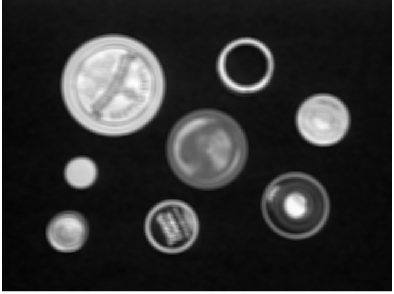
\includegraphics[width=0.5\textwidth]{part1.png}
\caption{Image smoothed with $9\times 9$ gaussian kernel with $\sigma=1$ }
\label{fig1}
\end{center}
\end{figure}

\begin{center}
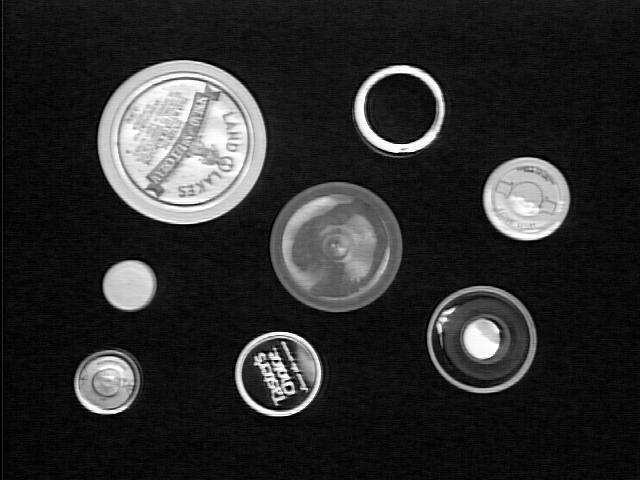
\includegraphics[width=0.3\textwidth]{original_grayscale_image.jpg}
\\original grayscale image
\end{center}

\newpage

\begin{figure}[htp]
    \centering
    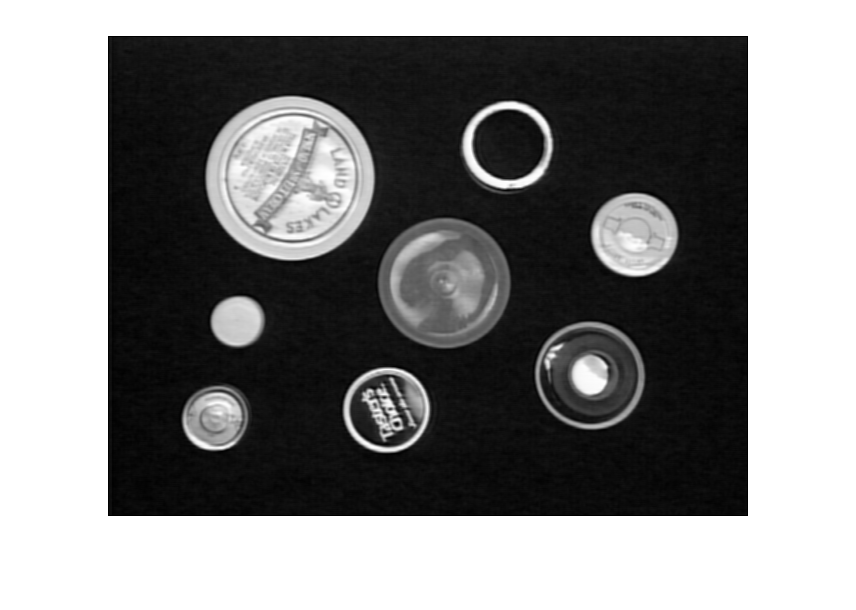
\includegraphics[width=6cm]{3X3 sigma-2.png} 
    3X3 sigma = 2
    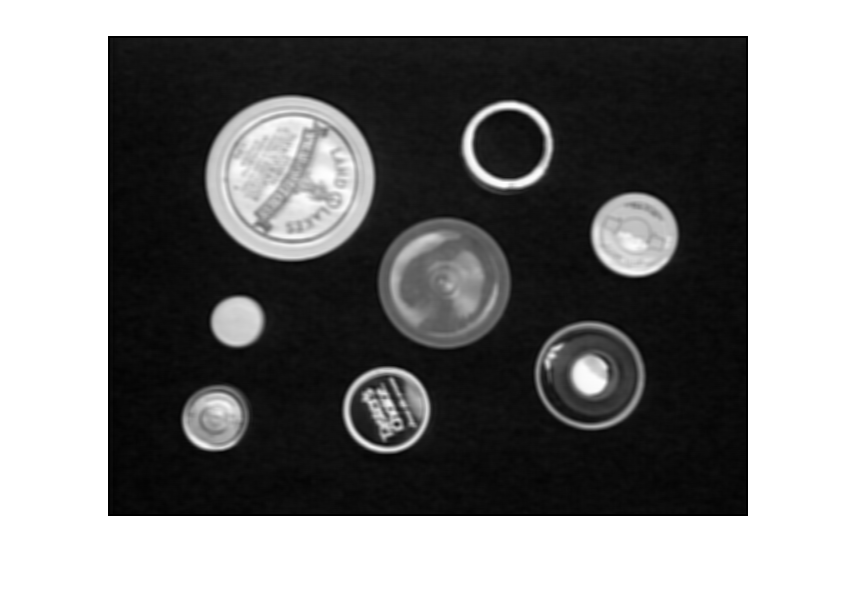
\includegraphics[width=6cm]{5X5 sigma-3.png} 
    5X5 sigma = 3
    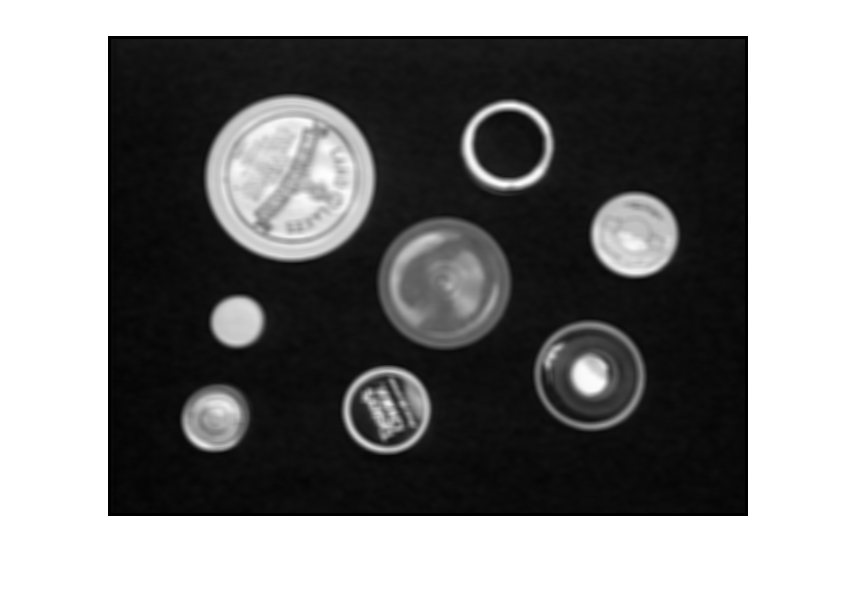
\includegraphics[width=6cm]{7X7 sigma-4.png} 
    7X7 sigma = 4
    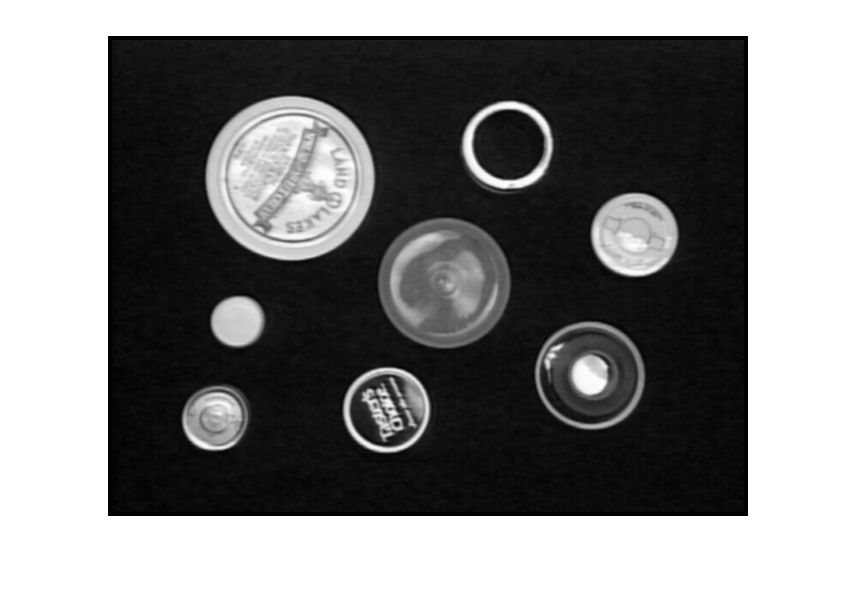
\includegraphics[width=6cm]{9X9 sigma-1.png} 
    9X9 sigma = 1
\end{figure}
    

\newpage
\section{Gradients}
Next, we’ll compute the gradients on our  image. \\

\noindent
Generate three images using the original image (not smoothed):
\begin{enumerate}
\item One which has the absolute value of the change with respect to the change in $x$
\item One that has the absolute value of the change with respect to the change in $y$
\item One that has the overall magnitude of the combined gradients.
\end{enumerate}

\noindent
Doing this on your original image you’ll likely see “noise”, so next try first applying a smoothing filter (like you developed in the previous part) to remove noise prior to extracting gradients.  You can choose the parameters of the kernel as you see fit.   Show these images as well (6 total images).\\

\noindent
An example of a gradient magnitude image can be found in Figure \ref{fig2}.

\begin{figure}[H]
\begin{center}
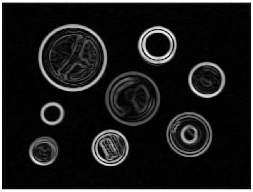
\includegraphics[width=0.5\textwidth]{part3.png}
\caption{Magnitude gradient image after smoothing.}
\label{fig2}
\end{center}
\end{figure}

\noindent
\emph{Note:}  Since you already demonstrated in the previous part your ability to perform convolution, for the remaining parts of the assignment you \textbf{may} use Matlab’s \emph{conv2} function. 

\newpage

three images using the original image\\

\begin{figure}[htp]
    \centering
    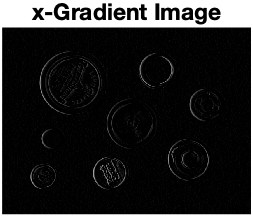
\includegraphics[width=5cm]{x.png}
    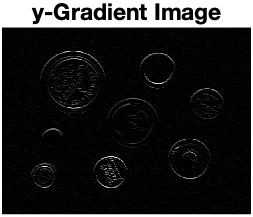
\includegraphics[width=5cm]{y.png}
    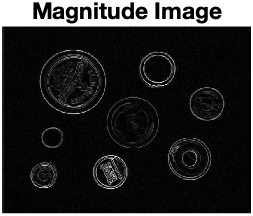
\includegraphics[width=5cm]{magnitude.png}
\end{figure}

to apply a smoothing filter to the original image and compute the gradients\\

\begin{figure}[htp]
    \centering
    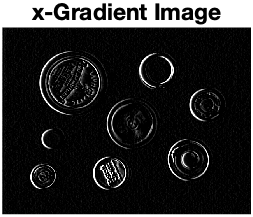
\includegraphics[width=5cm]{x-filter.png}
    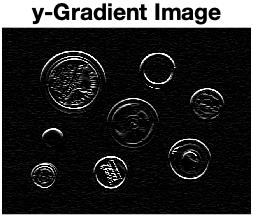
\includegraphics[width=5cm]{y-filter.png}
    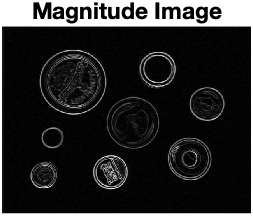
\includegraphics[width=5cm]{magnitude-filter.png}
\end{figure}

\newpage
\section{Non-maximum suppression}
Our next step is to apply \emph{non-maximum supression} to the gradient information.\\

\noindent
Using the gradient information, compute the magnitude and angle of the gradient for each pixel.   Then, for all pixels, compare the magnitude of the gradient of this pixel to two nearest neighbors, in the direction to and opposite the gradient direction, as defined in the table below.  If the magnitude of its gradient is the largest of those neighbors, flag it to continue through the pipeline.\\

\noindent
A few notes about doing this in Matlab:
\begin{itemize}
\item Use the $atan2$ function to get the angles.  This returns the \emph{four-quadrant atan} with values in the range of $[-\pi, \pi]$.  See the Matlab documentation for more details.
\end{itemize}

\begin{table}[h]
\centering
\begin{tabular}{|l|l|}
\hline
\textbf{Pixels to check} & \textbf{Angle}\\
\hline
Left and right & $ \theta<-\frac{7\pi}{8}$ or $\theta\geq\frac{7\pi}{8}$ or $-\frac{\pi}{8}\leq \theta < \frac{\pi}{8}$\\
Up and down & $-\frac{5\pi}{8}\leq\theta<-\frac{3\pi}{8}$ or $\frac{3\pi}{8}\leq\theta<\frac{5\pi}{8}$\\
Up-right and down-left* & $-\frac{3\pi}{8}\leq\theta<-\frac{\pi}{8}$ or $\frac{5\pi}{8}\leq\theta<\frac{7\pi}{8}$\\
Up-left and down-right* & $-\frac{7\pi}{8}\leq\theta<-\frac{5\pi}{8}$ or $\frac{1\pi}{8}\leq\theta<\frac{3\pi}{8}$\\
\hline
\end{tabular}
\end{table}


\noindent
* These may be counter-intuitive.  But since the y-axis is inverted for the image coordinate plane, the angles are reflected about the x-axis.\\

\noindent
An example can be found in Figure \ref{fig3}.

\begin{figure}[H]
\begin{center}
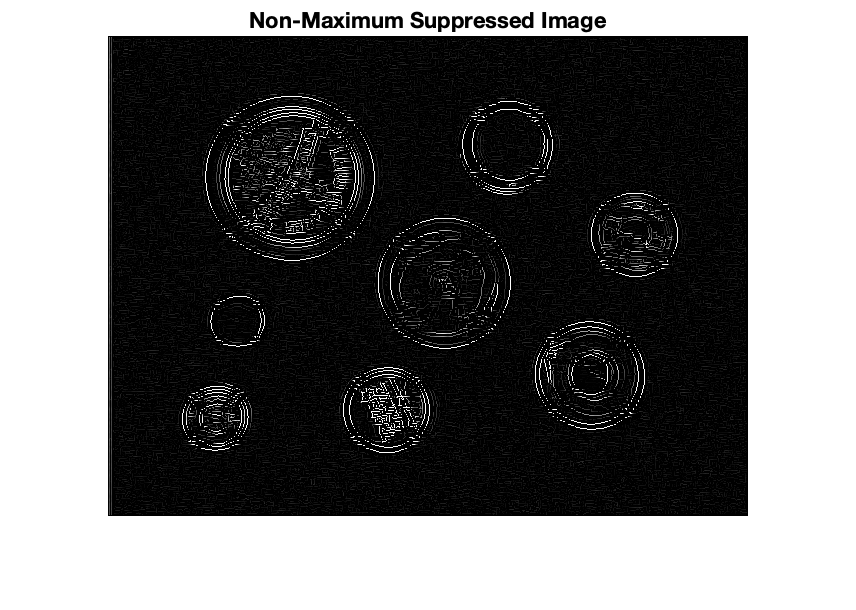
\includegraphics[width=0.5\textwidth]{nms_mag.png}
\caption{Gradient Magnitude after Non-Maximum Suppression.}
\label{fig3}
\end{center}
\end{figure}
\newpage
\section{Hysterisis}
For our final step, set a low and high threshold such that a pixel is an edge pixel if its gradient is greater than the high threshold, or if it is greater than the low threshold and borders (8-way) a pixel that is above the high threshold.  The result should be a \emph{binary} image.  Here you just need to provide one example output, but also report the parameter choices (smoothing kernel and thresholds).\\

\noindent
An example can be found in Figure \ref{fig4}.

\begin{figure}[H]
\begin{center}
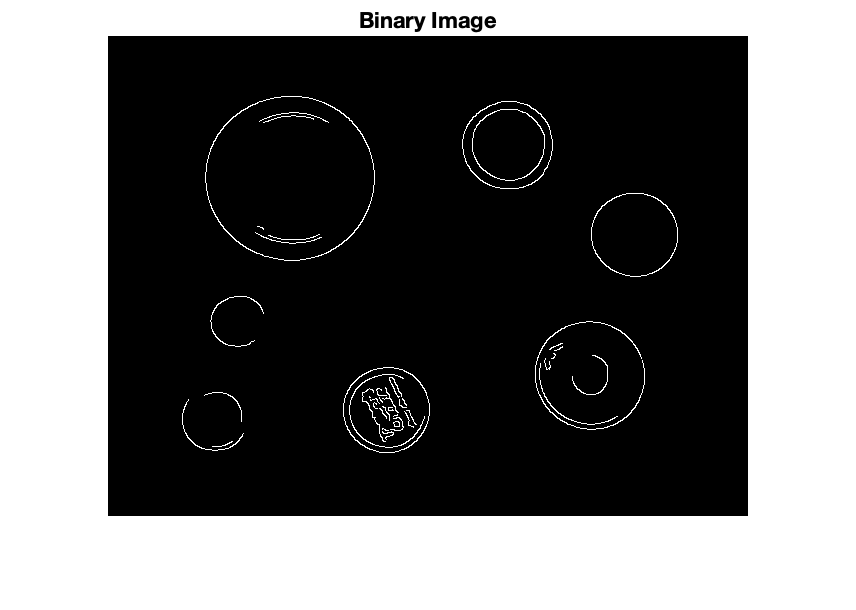
\includegraphics[width=0.5\textwidth]{hysteresis.png}
\caption{Hysteresis thresheld binary edge image.}
\label{fig4}
\end{center}
\end{figure}

\newpage
\section{Test on another image}
Now that you have all the stages of your Canny Edge Detector implemented, somehow obtain another image and apply your Canny Edge Detector to it.  Show the result as it goes through each part of the pipeline.\\

    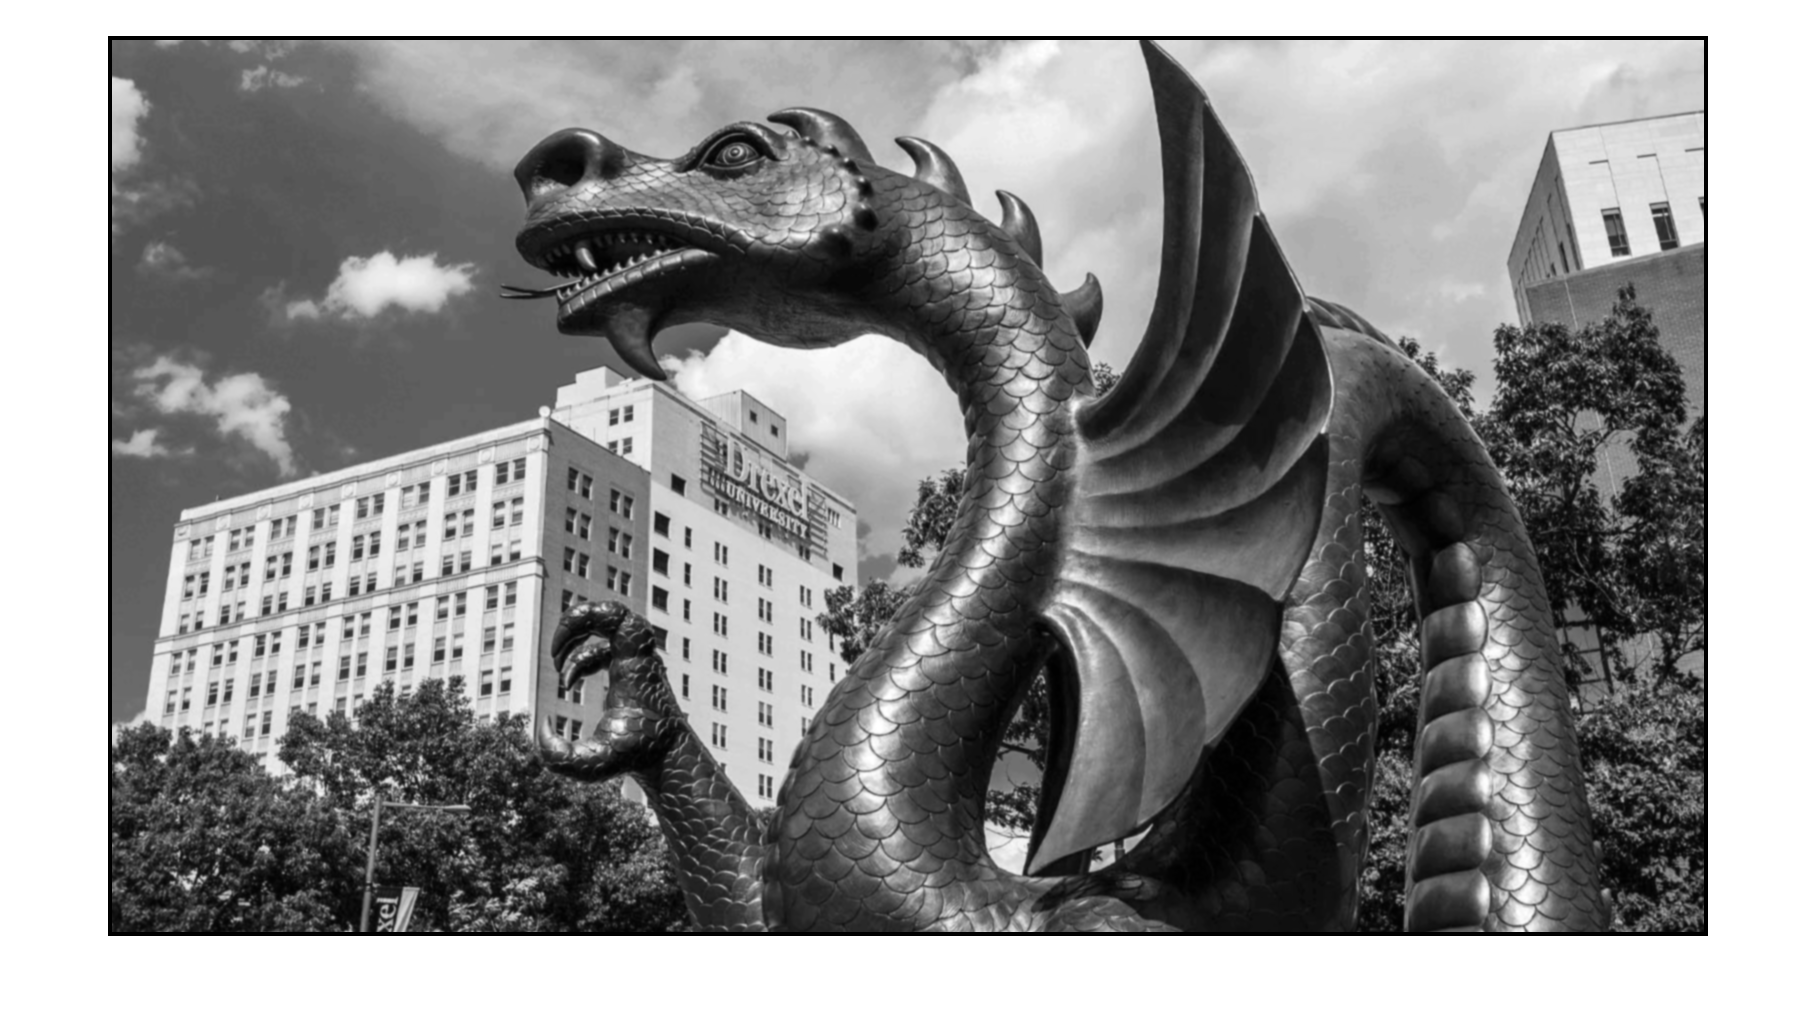
\includegraphics[width=7cm]{Smoothed image.png}
    Original image\\
    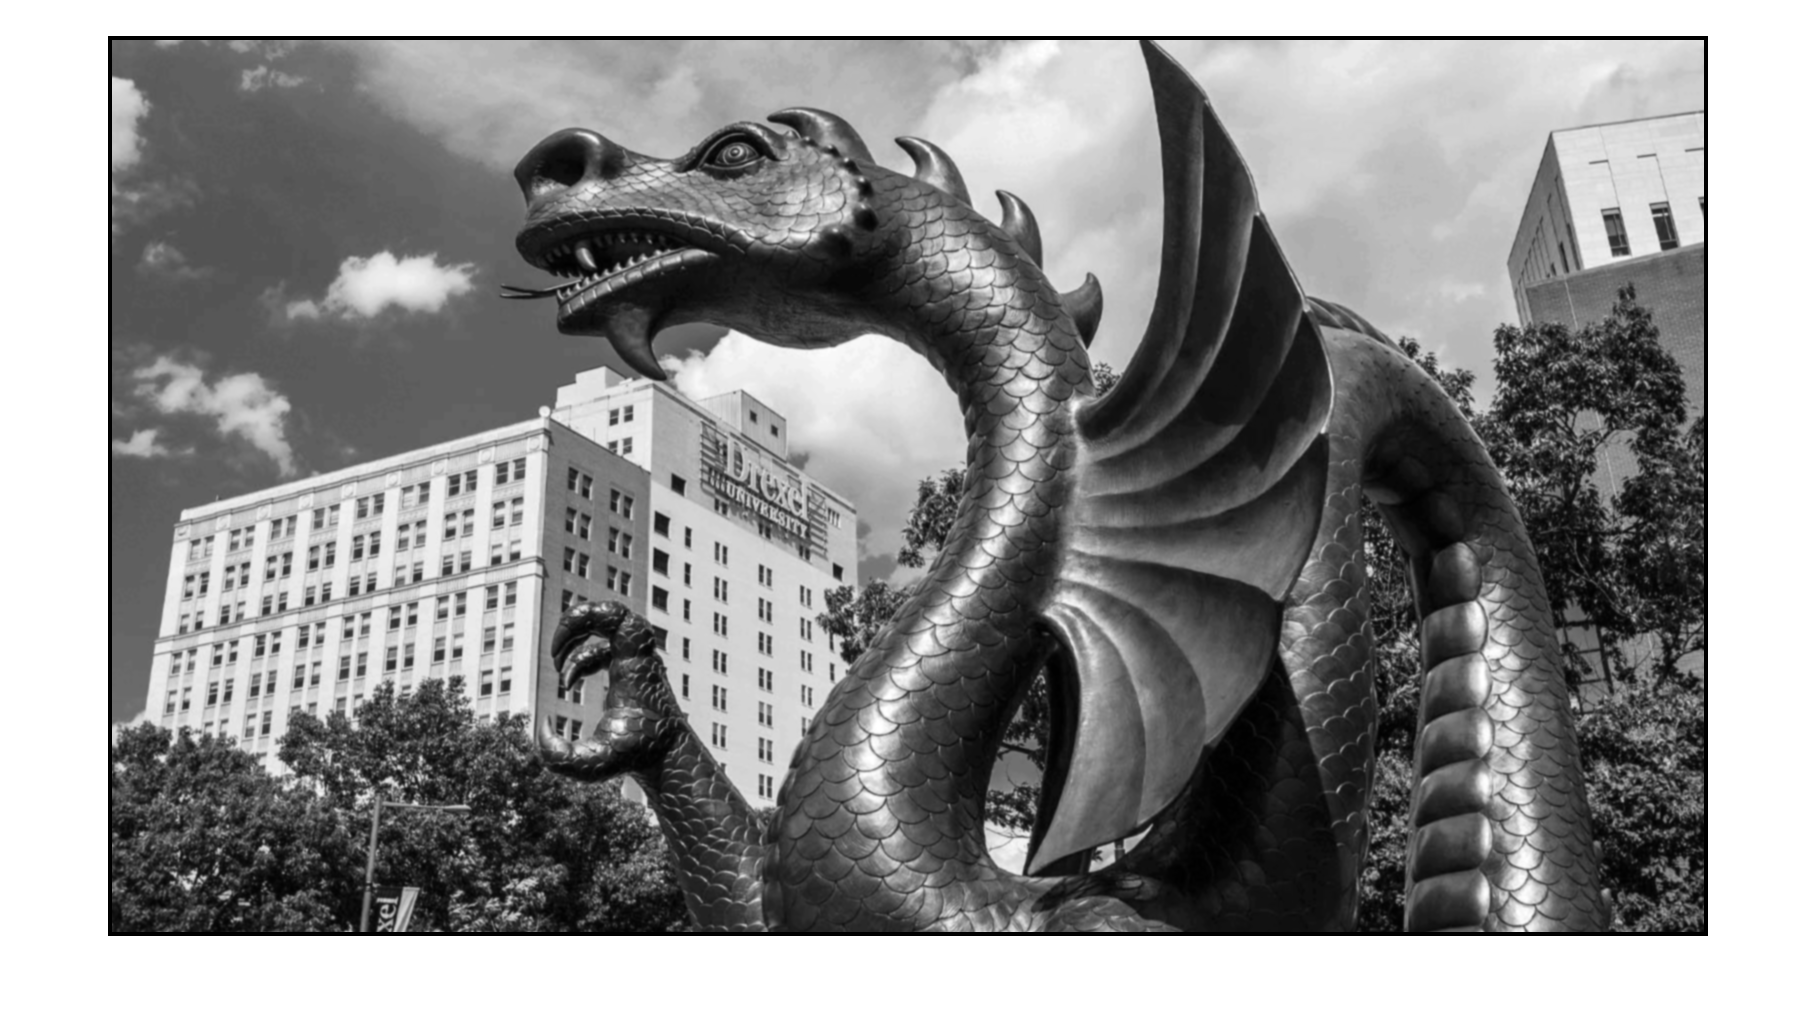
\includegraphics[width=7cm]{Smoothed image.png}
    Smoothed image\\
    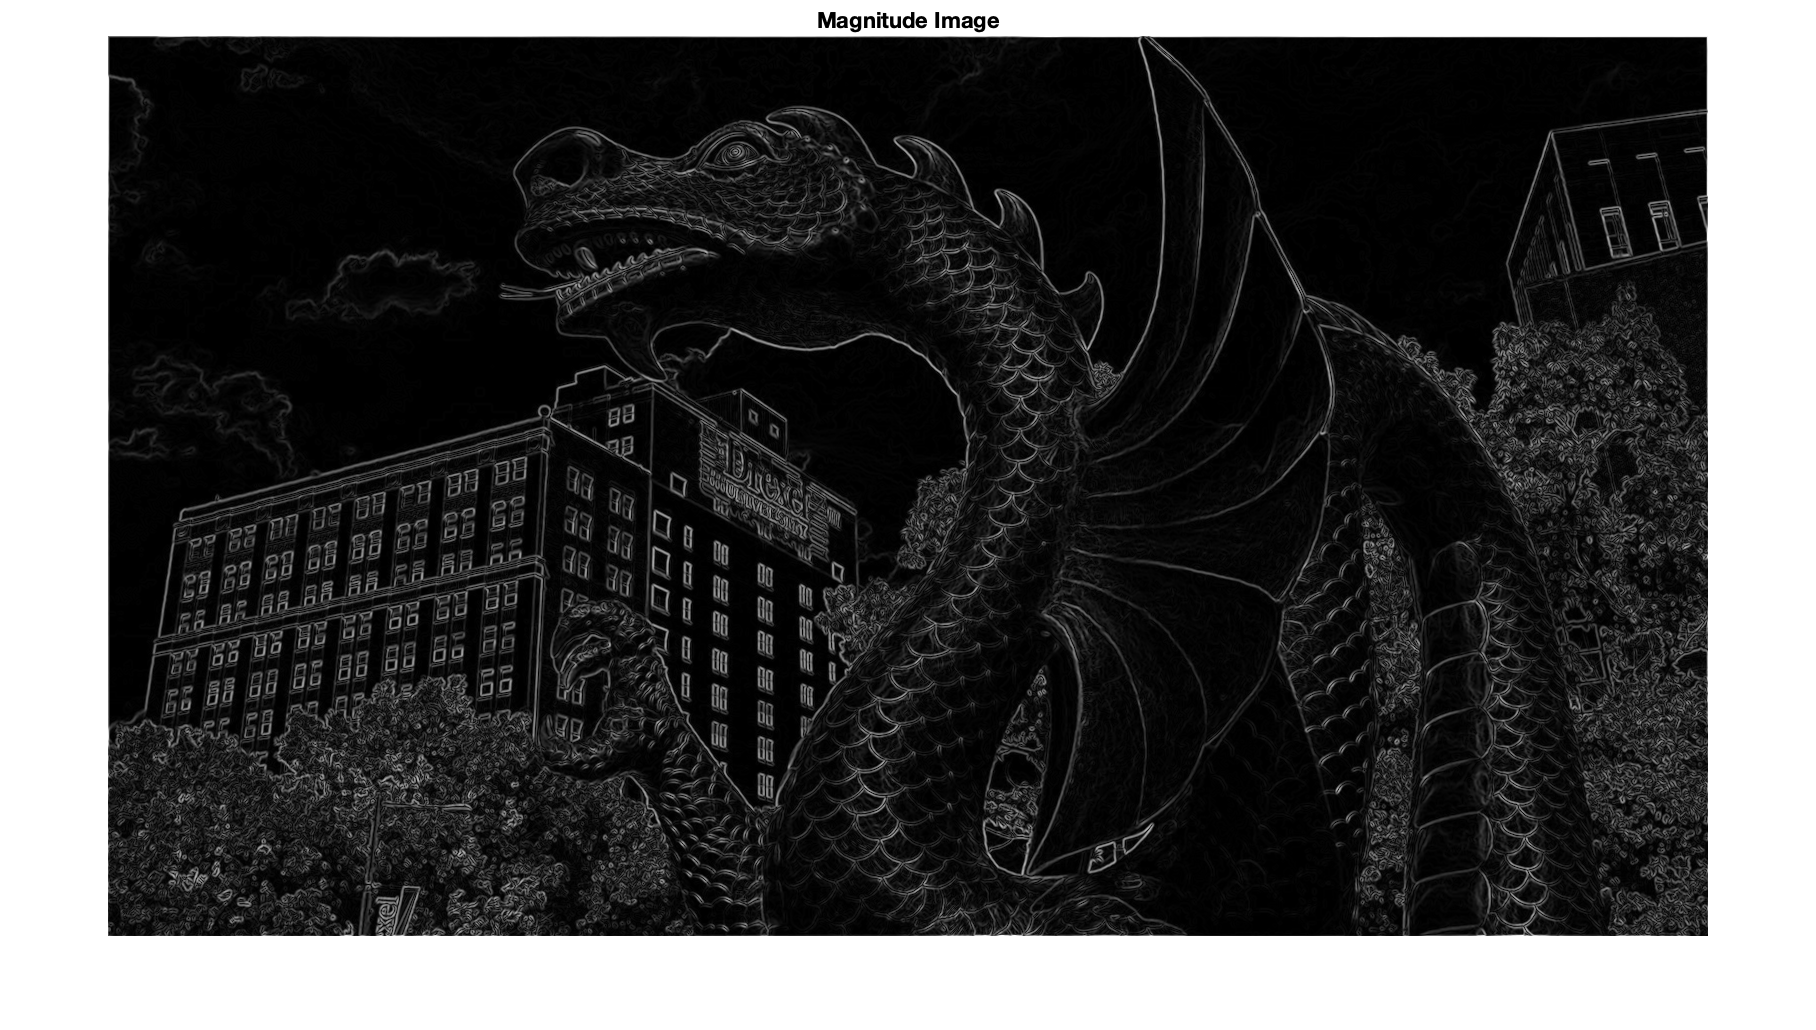
\includegraphics[width=7cm]{Gradient magnititude image.png}
    Gradient magnititude image\\
    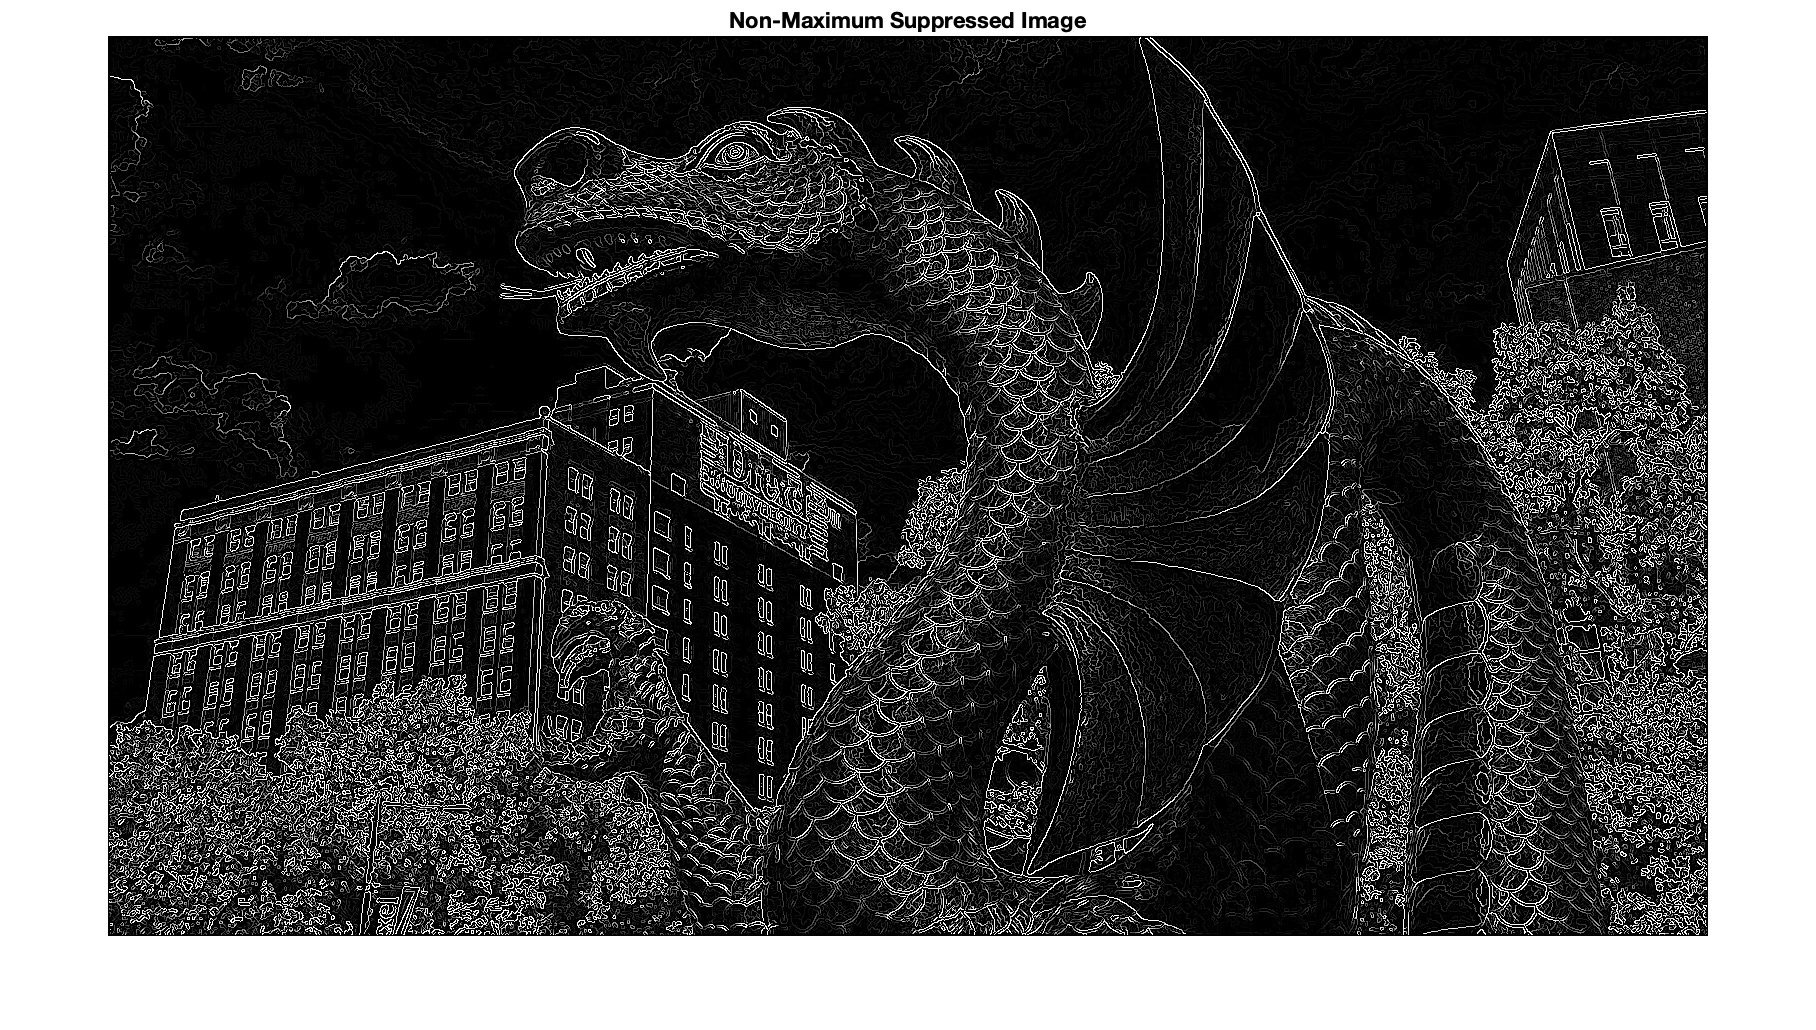
\includegraphics[width=7cm]{non-maximum suppression.png}
    non-maximum suppression\\
    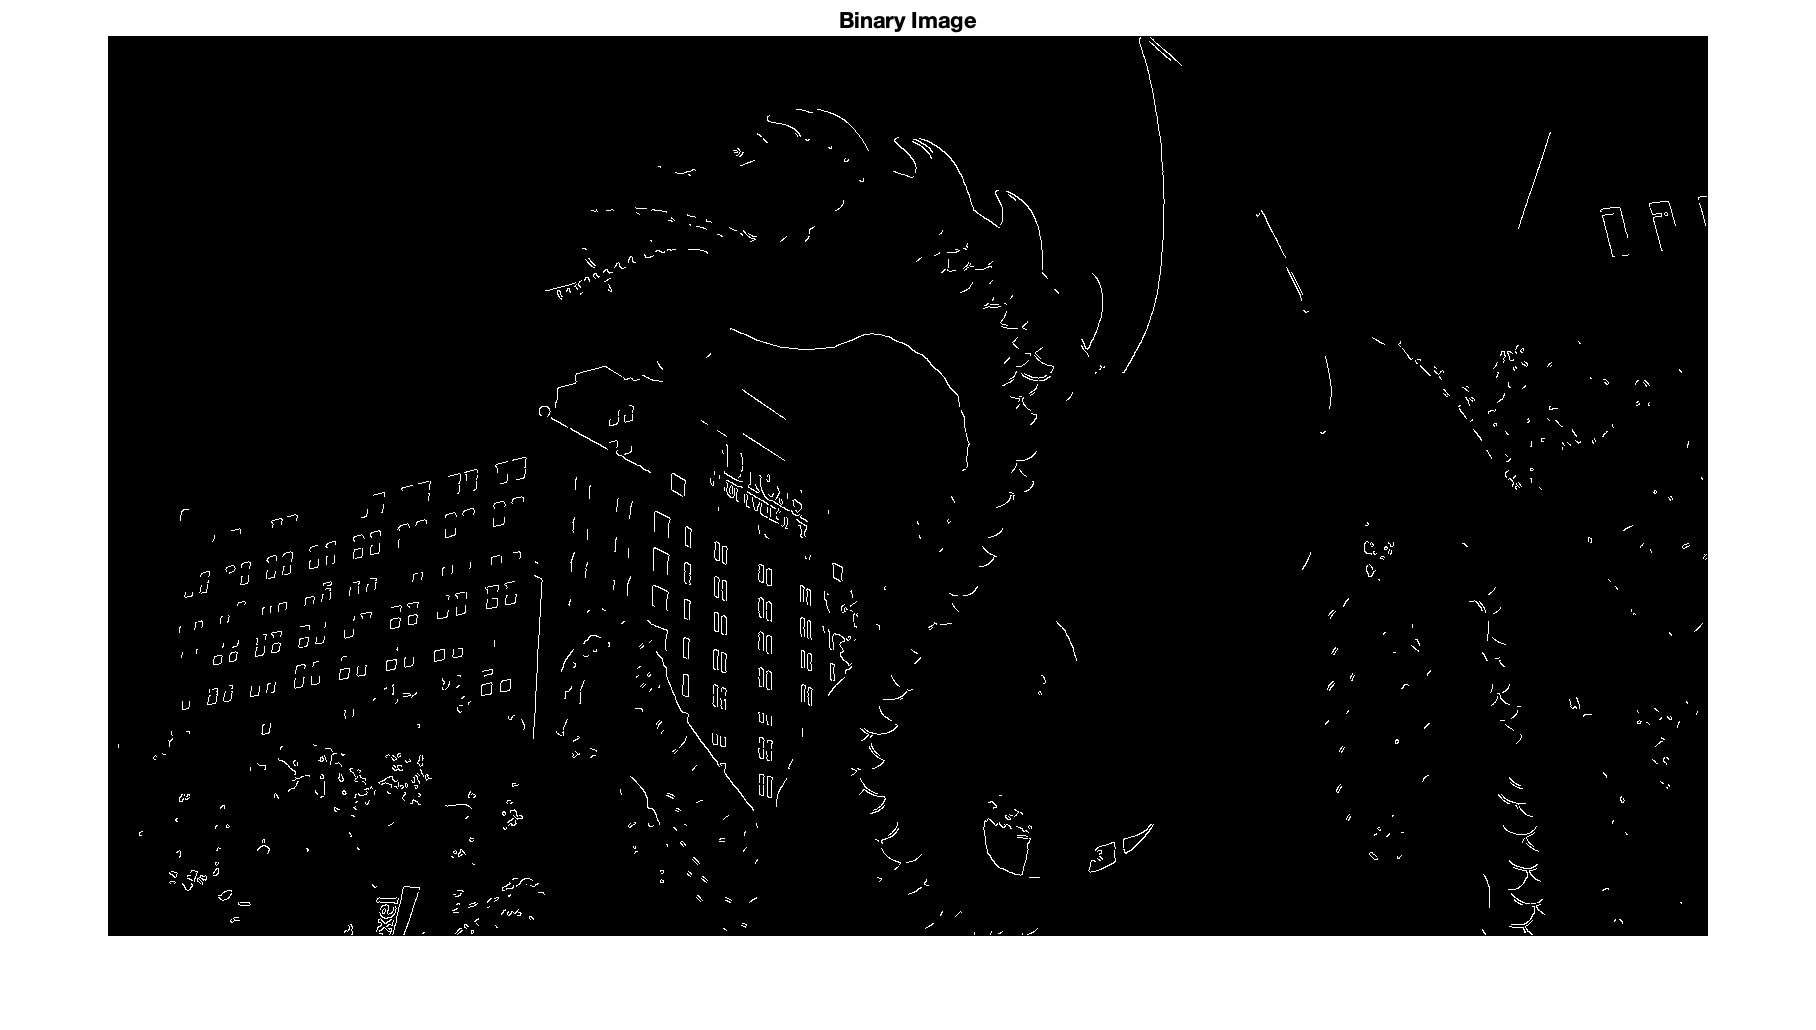
\includegraphics[width=7cm]{Hysterisis edge image.png}
    Hysterisis edge image\\



\newpage
\section*{Submission}
For your submission, upload to Blackboard a single zip file containing:

\begin{enumerate}
\item PDF writeup that includes:
\begin{enumerate}
\item Your answer to the theory question(s).
\item For Part 2, 5 images.  The original grayscale, then 4 combinations of the parameters $(N,\sigma)$.
\item For Part 3, 6 total images.  Three showing the partial gradients and magnitude of the gradient without pre-smoothing, and three after.  In addition, report the parameters of the kernel you used for smoothing.
\item For Part 4, your non-maximum suppressed image.
\item For Part 5, your binary edge image usng hysteresis.  In your report provide the parameters of the smoothing kernel and the low and high threshold values for the hysterisis process.
\item For Part 6, 5 total image:
	\begin{enumerate}
	\item Original image (either color or gray)
	\item Smoothed image (along with choice of smoothing filter parameters).
	\item Gradient magnititude image
	\item Hysterisis edge image (along with choice of thresholds)
	\item Final edge image with non-maximum suppression applied.
	\end{enumerate}
\end{enumerate}
\item A README text file (\textbf{not} Word or PDF) that explains:
\begin{enumerate}
\item Any unique features of your program (if applicable).
\item Any instructions on how to run your script to reproduce your results.
\end{enumerate}
\item Your source file(s).
\item The chosen image(s) that you processed.
\end{enumerate}

\end{document}

